
\section{encapsulation motivations}
\subsection{use case: on remote network}


\usetikzlibrary{arrows.meta,calc,patterns,shapes}
\providecommand{\computer}{%
    
\includegraphics[width=1cm]{../common/Noun_project_216.pdf}
}
\providecommand{\switch}{%
    
\includegraphics[width=0.9cm]{../common/fig-switch.pdf}
}
\providecommand{\bigswitch}{%
    
\includegraphics[width=1.4cm]{../common/fig-switch.pdf}
}
\providecommand{\router}{%
    
\includegraphics[width=0.9cm]{../common/fig-router.pdf}
}

\begin{frame}[label=connTwoNet]{on a remote network}
\begin{tikzpicture}
\tikzset{
    connect/.style={draw,very thick,Latex-Latex},
    computer/.style={inner sep=0mm,outer sep=0mm,execute at begin node={\computer}},
    switch/.style={inner sep=0mm,outer sep=0mm,execute at begin node={\switch}},
    big switch/.style={inner sep=0mm,outer sep=0mm,execute at begin node={\bigswitch}},
    router/.style={inner sep=0mm,outer sep=-2mm,execute at begin node={\router},circle},
    packet/.style={minimum width=.4cm,minimum height=0.2cm,inner sep=0mm,outer sep=0mm,draw},
    packet lg/.style={minimum width=.6cm,minimum height=0.2cm,inner sep=0mm,outer sep=0mm,draw},
    network/.style={draw,cloud,font=\small,aspect=3,inner sep=-.05cm},
    tunnel/.style={dotted,line width=1mm,dotted,blue,Latex-Latex,opacity=0.7},
}
\begin{scope}[xshift=0cm,yshift=1cm,name prefix=norm-]
    \node[computer] (comp) at (0, 0) {};
    \node[network,minimum height=1.7cm,minimum width=2.7cm] (internet) at (0, 3)  {
        internet
    };
    \node[network] (company) at (4, 2) {company};
    \node[draw,thick] (server) at (4, 0) {server};
    \foreach \x/\y in {comp/internet,internet/company,company/server} {
        \draw[connect] (\x) -- (\y);
    }
    \draw[tunnel]
        (comp.north) -- ([yshift=-.4cm,xshift=0cm]internet.center)
            -- ([yshift=-.0cm,xshift=1cm]internet.center) -- (company.center)
            -- (server.north);
\end{scope}
\node at (2, 6) { actual connections };
\node at (10, 6) { logical connections };
\draw[ultra thick] (6, -1) -- ++ (0, 7);
\begin{scope}[xshift=8cm,yshift=1cm,name prefix=alt-]
    \node[computer] (comp) at (0, 0) {};
    \node[network,minimum height=1.7cm,minimum width=2.7cm] (internet) at (0, 3)  {
        internet
    };
    \node[network] (company) at (4, 2) {company};
    \node[draw,thick] (server) at (4, 0) {server};
    \foreach \x/\y in {internet/company,company/server,comp/company} {
        \draw[connect] (\x) -- (\y);
    }
\end{scope}
\end{tikzpicture}
\end{frame}


\subsection{use case: connect networks}

\usetikzlibrary{arrows.meta,calc,patterns,shapes}
\providecommand{\computer}{%
    
\includegraphics[width=1cm]{../common/Noun_project_216.pdf}
}
\providecommand{\switch}{%
    
\includegraphics[width=0.9cm]{../common/fig-switch.pdf}
}
\providecommand{\bigswitch}{%
    
\includegraphics[width=1.4cm]{../common/fig-switch.pdf}
}
\providecommand{\router}{%
    
\includegraphics[width=0.9cm]{../common/fig-router.pdf}
}


\begin{frame}[label=connTwoNet]{connecting two networks}
\begin{tikzpicture}
\tikzset{
    connect/.style={draw,very thick,Latex-Latex},
    computer/.style={inner sep=0mm,outer sep=0mm,execute at begin node={\computer}},
    switch/.style={inner sep=0mm,outer sep=0mm,execute at begin node={\switch}},
    big switch/.style={inner sep=0mm,outer sep=0mm,execute at begin node={\bigswitch}},
    router/.style={inner sep=0mm,outer sep=-2mm,execute at begin node={\router},circle},
    packet/.style={minimum width=.4cm,minimum height=0.2cm,inner sep=0mm,outer sep=0mm,draw},
    packet lg/.style={minimum width=.6cm,minimum height=0.2cm,inner sep=0mm,outer sep=0mm,draw},
    network/.style={draw,cloud,font=\small,aspect=3,inner sep=-.25cm},
    tunnel/.style={dotted,line width=1mm,dotted,blue,Latex-Latex,opacity=0.7},
}
\begin{scope}
    \node[network] (site A) at (0, 0) {company site A};
    \node[network] (site B) at (4, 0) {company site B};
    \node[network,minimum height=1.7cm,minimum width=2.7cm] (internet) at (2, 4)  {
        internet
    };
    \node[router,anchor=south] (A route) at ([yshift=1cm]site A.north) {};
    \node[router,anchor=south] (B route) at ([yshift=1cm]site B.north) {};
    \foreach \x/\y in {site A/A route,site B/B route,A route/internet,B route/internet} {
        \draw[connect] (\x) -- (\y);
    }
    \draw[tunnel]
        (A route.north east) -- ([yshift=-.7cm,xshift=-1cm]internet.center)
            -- ([yshift=-.7cm,xshift=1cm]internet.center) -- (B route.north west);
    \node[draw=red,fill=white,align=center,anchor=north,font=\small,thick] at (2, 5.7) {
        setup tunnel \\
        between disconnected sites
    };
\end{scope}
\node at (2, 6) { actual connections };
\node at (10, 6) { logical connections };
\draw[ultra thick] (6, -1) -- ++ (0, 7);
\begin{scope}[xshift=8cm,name prefix=alt-]
    \node[network] (site A) at (0, 0) {company site A};
    \node[network] (site B) at (4, 0) {company site B};
    \node[network,minimum height=1.7cm,minimum width=2.7cm] (internet) at (2, 4)  {
        internet
    };
    \node[router,anchor=south] (A route) at ([yshift=1cm]site A.north) {};
    \node[router,anchor=south] (B route) at ([yshift=1cm]site B.north) {};
    \foreach \x/\y in {site A/A route,site B/B route,A route/internet,B route/internet} {
        \draw[connect] (\x) -- (\y);
    }
    \node[draw=red,align=center,fill=white,anchor=north,font=\small,thick] at (2, 5.7) {
        as if directly\\
        linked sites
    };
    \draw[connect] (A route) -- (B route);
\end{scope}
\end{tikzpicture}
\end{frame}



\subsection{use case: two networks}


\usetikzlibrary{arrows.meta,calc,patterns,shapes}
\providecommand{\computer}{%
    
\includegraphics[width=1cm]{../common/Noun_project_216.pdf}
}
\providecommand{\switch}{%
    
\includegraphics[width=0.9cm]{../common/fig-switch.pdf}
}
\providecommand{\bigswitch}{%
    
\includegraphics[width=1.4cm]{../common/fig-switch.pdf}
}
\providecommand{\router}{%
    
\includegraphics[width=0.9cm]{../common/fig-router.pdf}
}


\begin{frame}[label=connTwoNet]{two networks in one}
\begin{tikzpicture}
\tikzset{
    connect/.style={draw,very thick,Latex-Latex},
    computer/.style={inner sep=0mm,outer sep=0mm,execute at begin node={\computer}},
    phone/.style={draw,thin,font=\tiny,inner sep=0mm,outer sep=0mm,execute at begin node={phone}},
    switch/.style={inner sep=0mm,outer sep=0mm,execute at begin node={\switch}},
    big switch/.style={inner sep=0mm,outer sep=0mm,execute at begin node={\bigswitch}},
    router/.style={inner sep=0mm,outer sep=-2mm,execute at begin node={\router},circle},
    packet/.style={minimum width=.4cm,minimum height=0.2cm,inner sep=0mm,outer sep=0mm,draw},
    packet lg/.style={minimum width=.6cm,minimum height=0.2cm,inner sep=0mm,outer sep=0mm,draw},
    network/.style={draw,cloud,font=\small,aspect=3,inner sep=-.25cm},
    tunnel/.style={dotted,line width=1mm,dotted,blue,Latex-Latex,opacity=0.7},
}
\begin{scope}
    \node[switch,anchor=south] (switch A) at (2,3) {};
    \node[switch,anchor=south] (switch B) at (4,3) {};
    \node[computer] (c1) at (0,0) {};
    \node[phone] (p1) at (1,0) {};
    \node[computer] (c2) at (2,0) {};
    \node[phone] (p2) at (3,0) {};
    \node[computer] (c3) at (4,0) {};
    \foreach \x/\y in {c1,p1,c2} {
        \draw[connect] (\x) -- (switch A);
    }
    \foreach \x/\y in {p2,c3} {
        \draw[connect] (\x) -- (switch B);
    }
    \draw[connect] (switch A) -- (switch B);
\end{scope}
\node at (2, 6) { actual connections };
\node at (10, 6) { logical connections };
\draw[ultra thick] (6, -1) -- ++ (0, 7);
\begin{scope}[xshift=8cm,name prefix=alt-]
    \node[switch,anchor=south] (switch A) at (2,3) {};
    \node[switch,anchor=south] (switch B) at (4,3) {};
    \node[computer] (c1) at (0,0) {};
    \node[phone] (p1) at (1,0) {};
    \node[computer] (c2) at (2,0) {};
    \node[phone] (p2) at (3,0) {};
    \node[computer] (c3) at (4,0) {};
    \foreach \x/\y in {c1,c2,c3} {
        \draw[connect] (\x) -- (switch A);
    }
    \foreach \x/\y in {p1,p2} {
        \draw[connect] (\x) -- (switch B);
    }
\end{scope}
\end{tikzpicture}
\end{frame}



%FIXME: use-case: multiple networks

\subsection{summary/additional}
\begin{frame}{encapsulation: why? (1)}
    \begin{itemize}
    \item some possible scnearios (1/2):
    \vspace{.5cm}
    \item add encryption/authentication to data in flight
    \item be ``on University/company network'' from home
    \item hide original location of Internet connection
    \item make virtual machines running on different servers appear to be plugged into one switc
    \end{itemize}
\end{frame}

\begin{frame}{encapsulation: why? (2)}
    \begin{itemize}
    \item some possible scnearios (2/2):
    \vspace{.5cm}
    \item evade overally restrictive firewall rules
    \item make two datacenters connected via Internet appear to be one big network
    \item `separate' networks for phones v. desktops without buying two sets of switches
    \end{itemize}
\end{frame}



\subsection{aside: encryption via encapsulation}
\begin{frame}{aside: non-end-to-end encryption?}
    \begin{itemize}
    \item often encapsulation used to have encrypted link
    \item nice, but really want to encrypt between end-hosts
        \begin{itemize}
        \item example: SSH, HTTPS
        \end{itemize}
    \item exercise: extra vulnerable points if relying on encrypted link idea?
    \end{itemize}
\end{frame}


% FIXME: use-case: two networks

% FIXME: split out other motivations

\section{encapsulation options, generally}
\begin{frame}{encapsulation options [incomplete]}
\small
\begin{tabular}{l||p{4cm}|p{4cm}|p{2cm}}
left in above       & TCP/UDP/higher layers & IP & link-layer \\ \hline \hline
above TCP/UDP       & HTTP proxy, DNS over HTTP(S) & --- & --- \\ \hline
TCP/UDP             & SOCKS, HTTP CONNECT, SSH conn forwarding, TLS & --- & --- \\\hline
IP                  & OpenVPN, WireGuard & GRE, IPsec & MPLS \\\hline
link-layer          & OpenVPN, \ldots & ? & VLAN, MPLS \\\hline
\end{tabular}
\end{frame}

\begin{frame}{encapsulation steps}
    \begin{itemize}
    \item 1. getting the stuff to encapsulate
    \item 2. sending it encapsulated
    \vspace{.5cm}
    \item will start by focusing on first problem
    \end{itemize}
\end{frame}

\begin{frame}[label=encapChanges]{encapsulating w/ app changes}
    \begin{itemize}
    \item application might have special code to handle connecting differently
    \item + might take advantage of extra information in encapsulation
    \vspace{.5cm}
    \item example: many application's TLS support
    \item example: web browser HTTP/SOCKS proxy support
    \end{itemize}
\end{frmae}

\begin{frame}<2>[label=encapChanges]{encapsulating w/o app changes}
\begin{itemize}
\item generally: easier to do for lower layers
\vspace{.5cm}
\item link-layer in something
    \begin{itemize}
    \item \myemph<2>{``virtual'' (probably Ethernet) device}
    \item \myemph<2>{sends/receives from `tunnel'}
    \end{itemize}
\item IP in something
    \begin{itemize}
    \item \myemph<3>{``virtual'' IP link}
    \item \myemph<3>{destination routing table can go to}
    \end{itemize}
\item UDP/TCP in something
    \begin{itemize}
    \item \myemph<4>{replace socket API}
    \item \myemph<5>{convince application to connect to different IP address?}
    \item \myemph<6>{use virtual IP link + implement one end of TCP/UDP}
    \end{itemize}
\end{itemize}
\end{frame}

\againframe<2>{encapChanges}

\begin{frame}[fragile]{Linux tap devices}
\begin{Verbatim}[fontsize=\fontsize{10}{11}]
# create virtual ethernet device mydev
$ ip tuntap add dev mydev mode tap
# mark ethernet device as up
$ ip link set mydev up
$ dhclient mydev # or other commands to use/config device
\end{Verbatim}
(dhclient is a DHCP client) \\
---
\begin{Verbatim}[fontsize=\fontsize{10}{11}]
int opentap(const char * name) {
    ... /* setup code, not shown*/
}
...
int fd = opentap("mydev");
...
write(fd, ethernetPacket, packetSize)
/* and (probably in separate threads) */
read(fd, buffer, SIZE); processEthernetPacket(buffer);
\end{Verbatim}
\end{frame}

\againframe<3>{encapChanges}

\begin{frame}[fragile]{Linux tun devices}
    \begin{itemize}
    \item same as `tap' devices, but\ldots
    \item get IP packets, not ethernet packets
    \end{itemize}
\begin{Verbatim}[fontsize=\fontsize{10}{11}]
# create virtual ethernet device mydev
$ ip tuntap add dev mydev mode tun
# setup device to be routed to, example:
$ ip address add 10.0.0.2 dev mydev
$ ip route add 10.0.0.0/24 dev mydev
$ ip -6 address add 3fff:1234::1 dev mydev
$ ip -6 route add 3fff:1234::/32 dev mydev
\end{Verbatim}
    \begin{itemize}
    \item tunneling program can then open device and read/write IP packets
    \end{itemize}
\end{frame}

\begin{frame}[fragile]{full tunnel routing table}
say 198.51.100.5 is running tunnel sever, \\
and 10.0.2.5  is gateway beyond tunnel, \\
and 203.0.113.54 is local gateway: \\
\begin{tabular}{l|l|l|l}
address & next hop & dev & priority\\ \hline
10.0.2.0/24 & --- & tunnel & normal \\
198.51.100.5/32 & 208.0.113.54 & real & high\\
(default) & 203.0.113.54 & real & normal \\
(default) & 10.0.2.5 & tunnel & high \\
\end{tabular}
\end{frame}


\begin{frame}[fragile]{split tunnel routing table}
say 198.51.100.5 is running tunnel sever, \\
and 10.0.2.5  is gateway beyond tunnel, \\
and 10.0.0.0/16, 198.51.100.0/24 are tunneled networks \\
and 203.0.113.54 is local gateway: \\
\begin{tabular}{l|l|l|l}
address & next hop & dev & priority\\ \hline
10.0.2.0/24 & --- & tunnel & normal \\
10.0.0.0/16 & 10.0.2.5& tunnel & normal \\
198.51.100.0/24 & 10.0.2.5& tunnel & normal \\
198.51.100.5/32 & 208.0.113.54 & real & high\\
(default) & 203.0.113.54 & real & normal \\
\end{tabular}
\end{frame}

\againframe<4>{encapChanges}

\begin{frame}[fragile]{`transparent' proxy (1)}
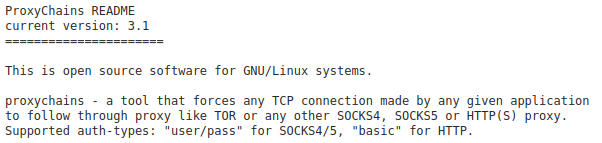
\includegraphics[width=\textwidth]{../encap/proxy-chains}
\begin{itemize}
\item configures dynamic library loader to load its library
    \begin{iteimze}
    \item \texttt{LD\_PRELOAD}
    \end{itemize}
\item with special versions of \texttt{connect}
\end{itemize}
\end{frame}

\againframe<5>{encapChanges}

\begin{frame}
    \begin{itemize}
    \item example: \texttt{stunnel} for `tunneling' TCP in TLS
    \item run on port X, configure to connect to some remote host
    \item configure non-TLS-aware program to connect to localhost port X
    \item \ldots instead of remote host
    \end{itemize}
\end{frame}

\againframe<6>{encapChanges}

\begin{frame}{ethernet to socket translation?}
    \begin{itemize}
    \item know of programs that capture Ethernet, extract socket() operations
    \item examples: slirp, passt
    \item current main use:
        \begin{itemize}
        \item networking for virtual machines \ldots
        \item \ldots without permission to configure new virtual network devices
        \end{itemize}
    \vspace{.5cm}
    \item but these don't support then tunneling the TCP/UDP connections
        \begin{itemize}
        \item instead just make normal socket calls
        \end{itemize}
    \end{itemize}
\end{frame}

\begin{frame}
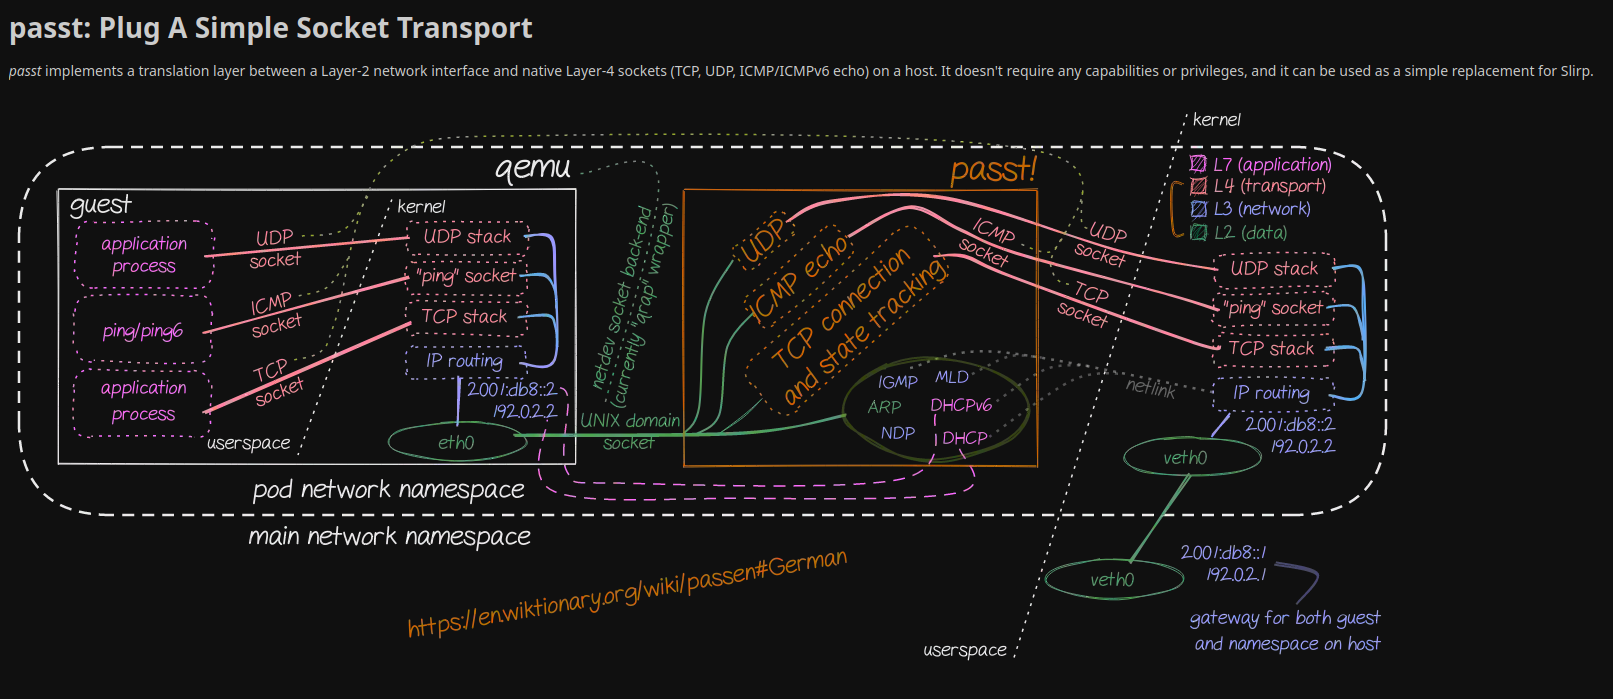
\includegraphics[width=\textwidth]{../encap/passt}
\end{frame}


\subsection{capturing packets}
\againframe<2>{encapSteps}
\begin{frame}[label=encapChanges]{encapsulating w/ app changes}
    \begin{itemize}
    \item application might have special code to handle connecting differently
    \item + might take advantage of extra information in encapsulation
    \vspace{.5cm}
    \item example: many application's TLS support
    \item example: web browser HTTP/SOCKS proxy support
    \end{itemize}
\end{frame}

\begin{frame}<2>[label=encapChanges]{encapsulating w/o app changes}
\begin{itemize}
\item generally: easier to do for lower layers
\vspace{.5cm}
\item link-layer in something
    \begin{itemize}
    \item \myemph<2>{``virtual'' (probably Ethernet) device}
    \item \myemph<2>{sends/receives from `tunnel'}
    \end{itemize}
\item IP in something
    \begin{itemize}
    \item \myemph<3>{``virtual'' IP link}
    \item \myemph<3>{destination routing table can go to}
    \end{itemize}
\item UDP/TCP in something
    \begin{itemize}
    \item \myemph<4>{replace socket API}
    \item \myemph<5>{convince application to connect to different IP address?}
    \item \myemph<6>{terminate UDP/TCP connection at `wrong' machine}
    \end{itemize}
\end{itemize}
\end{frame}

\againframe<2>{encapChanges}

\begin{frame}[fragile]{Linux tap devices}
\begin{Verbatim}[fontsize=\fontsize{10}{11}]
# create virtual ethernet device mydev
$ ip tuntap add dev mydev mode tap
# mark ethernet device as up
$ ip link set mydev up
$ dhclient mydev # or other commands to use/config device
\end{Verbatim}
(dhclient is a DHCP client) \\
---
\begin{Verbatim}[fontsize=\fontsize{10}{11}]
int opentap(const char * name) {
    ... /* setup code, not shown*/
}
...
int fd = opentap("mydev");
...
write(fd, ethernetPacket, packetSize)
/* and (probably in separate threads) */
read(fd, buffer, SIZE); processEthernetPacket(buffer);
\end{Verbatim}
\end{frame}

\againframe<3>{encapChanges}

\begin{frame}[fragile]{Linux tun devices}
    \begin{itemize}
    \item same as `tap' devices, but\ldots
    \item get IP packets, not ethernet packets
    \end{itemize}
\begin{Verbatim}[fontsize=\fontsize{12}{13}]
# create virtual ethernet device mydev
$ ip tuntap add dev mydev mode tun
# setup device to be routed to, example:
$ ip address add 10.0.0.2 dev mydev
$ ip route add 10.0.0.0/24 dev mydev
$ ip -6 address add 3fff:1234::1 dev mydev
$ ip -6 route add 3fff:1234::/32 dev mydev
\end{Verbatim}
    \begin{itemize}
    \item tunneling program can then open device and read/write IP packets
    \end{itemize}
\end{frame}

\begin{frame}[fragile]{full tunnel routing table}
say 198.51.100.5 is running tunnel sever, \\
and 10.0.2.5  is gateway beyond tunnel, \\
and 203.0.113.54 is local gateway: \\
\begin{tabular}{l|l|l|l}
address & next hop & dev & priority\\ \hline
10.0.2.0/24 & --- & tunnel & normal \\
198.51.100.5/32 & 208.0.113.54 & real & high\\
(default) & 203.0.113.54 & real & normal \\
(default) & 10.0.2.5 & tunnel & high \\
\end{tabular}
\end{frame}

\begin{frame}{alternate idea}
    \begin{itemize}
    \item shown: creating special route for tunnel destination
    \item alternate idea: tell OS to use correct interface/IP address
    \item most OSes: which IP address is bound = which network interface to use
        \begin{itemize}
        \item but would need to discover correct IP address
        \item might be tricky if wireless + wifi connections, or wifi changes
        \end{itemize}
    \end{itemize}
\end{frame}


\begin{frame}[fragile]{split tunnel routing table}
say 198.51.100.5 is running tunnel sever, \\
and 10.0.2.5  is gateway beyond tunnel, \\
and 10.0.0.0/16, 198.51.100.0/24 are tunneled networks \\
and 203.0.113.54 is local gateway: \\
\begin{tabular}{l|l|l|l}
address & next hop & dev & priority\\ \hline
10.0.2.0/24 & --- & tunnel & normal \\
10.0.0.0/16 & 10.0.2.5& tunnel & normal \\
198.51.100.0/24 & 10.0.2.5& tunnel & normal \\
198.51.100.5/32 & 208.0.113.54 & real & high\\
(default) & 203.0.113.54 & real & normal \\
\end{tabular}
\end{frame}

\againframe<4>{encapChanges}

\begin{frame}[fragile]{`transparent' proxy via library}
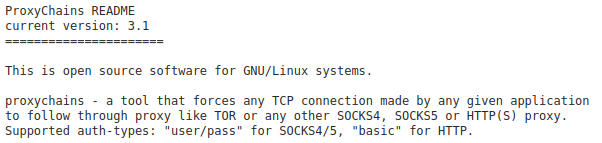
\includegraphics[width=\textwidth]{../encap/proxy-chains}
\begin{itemize}
\item configures dynamic library loader to load its library
    \begin{itemize}
    \item \texttt{LD\_PRELOAD}
    \end{itemize}
\item with special versions of \texttt{connect}
\end{itemize}
\end{frame}

\againframe<5>{encapChanges}

\begin{frame}{socket-in-socket}
    \begin{itemize}
    \item example: SSH connection forwarding
        \begin{itemize}
        \item \texttt{ssh -L X:remotehost:remoteport hostname}
        \end{itemize}
    \item example: \texttt{stunnel} for `tunneling' TCP in TLS
    \item run on port X, configure to connect to some remote host
    \item configure program to connect to localhost port X
    \item \ldots instead of remote host
    \end{itemize}
\end{frame}

\againframe<6>{encapChanges}

\begin{frame}[fragile]{`transparent' proxy via IP interception}
    \begin{itemize}
    \item example use case: shared HTTP cache used automatically
        \begin{itemize}
        \item if company/ISP wants everyone to use cache for performance
        \item if company wants to audit all HTTP proxy
        \end{itemize}
    \item configure router/firewall to diret all HTTP TCP connections to proxy
    \item either:
        \begin{itemize}
        \item configure proxy machine to accept connections on all IP addresses \textit{or}
        \item have router/firewall do network address translation (other direction)
        \end{itemize}
    \item HTTP proxy \texttt{squid} on Linux, some firewall boxes support this mode
    \item I don't think this is a good idea\ldots
        \begin{itemize}
        \item problematic with encryption
        \item proxy won't support newer HTTP stuff
        \end{itemize}
    \end{itemize}
\end{frame}



\section{sending encapsulated}
\againframe<3>{encapSteps}

\subsection{transport layer granularity}

\againframe<3>{encapOpt}

\subsection{SOCKS}
\usetikzlibrary{arrows.meta}
\begin{frame}{SOCKS (RFC 1928)}
    \begin{itemize}
    \item SOCKS motivation in RFC: firewall traversal
    \item supports both TCP and UDP
    \end{itemize}
\end{frame}

\begin{frame}{SOCKS TCP operation (client)}
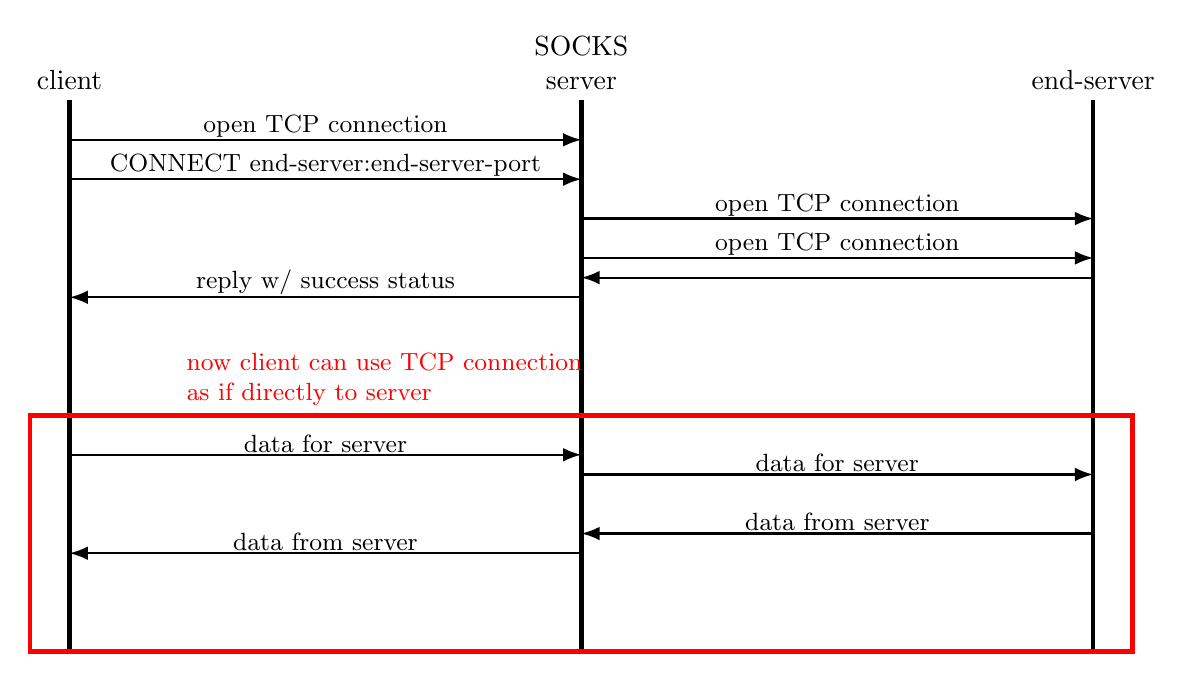
\begin{tikzpicture}
\begin{scope}[ultra thick]
    \draw (0, 0) node[above] {client} -- ++(0, -7);
    \draw (6.5, 0) node[above,align=center] {SOCKS\\server} -- ++(0, -7);
    \draw (13, 0) node[above] {end-server} -- ++(0, -7);
\end{scope}
\tikzset{
    msg/.style={font=\small,inner sep=0.2mm},
    send/.style={thick,-Latex},
}
\draw[send] (0, -.5) -- ++(6.5, 0) node[midway,above,msg] {open TCP connection};
%\draw[send] (6.5, -.75) -- ++(6.5, 0);
\draw[send] (0, -1) -- ++(6.5, 0) node[midway,above,msg] {CONNECT end-server:end-server-port};
\draw[send] (6.5, -1.5) -- ++(6.5, 0) node[midway,above,msg] {open TCP connection};
\draw[send] (6.5, -2) -- ++(6.5, 0) node[midway,above,msg] {open TCP connection};
\draw[send] (13, -2.25) -- ++(-6.5, 0);
\draw[send] (6.5, -2.5) -- ++(-6.5, 0) node[midway,above,msg] {reply w/ success status};
%
\draw[ultra thick,red] (-.5, -4) rectangle (13.5, -7);
\node[align=left,anchor=south,font=\small,red] at (4, -4) {
    now client can use TCP connection \\ as if directly to server
};
\draw[send] (0, -4.5) -- ++(6.5, 0) node[midway,above,msg] {data for server};
\draw[send] (6.5, -4.75) -- ++(6.5, 0) node[midway,above,msg] {data for server};
\draw[send] (13, -5.5) -- ++(-6.5, 0) node[midway,above,msg] {data from server};
\draw[send] (6.5, -5.75) -- ++(-6.5, 0) node[midway,above,msg] {data from server};
\end{tikzpicture}
\end{frame}

\begin{frame}{SOCKS TCP operation (server)}
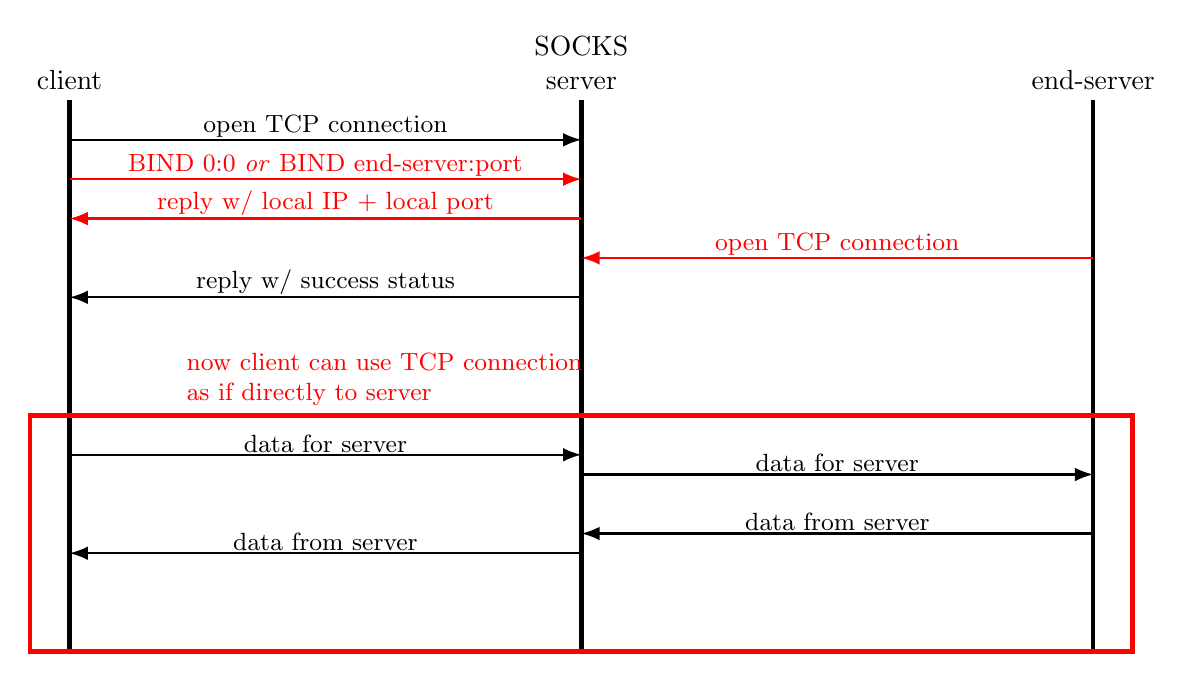
\begin{tikzpicture}
\begin{scope}[ultra thick]
    \draw (0, 0) node[above] {client} -- ++(0, -7);
    \draw (6.5, 0) node[above,align=center] {SOCKS\\server} -- ++(0, -7);
    \draw (13, 0) node[above] {end-server} -- ++(0, -7);
\end{scope}
\tikzset{
    msg/.style={font=\small,inner sep=0.2mm},
    send/.style={thick,-Latex},
    send misc/.style={thick,dotted,-Latex},
}
\draw[send] (0, -.5) -- ++(6.5, 0) node[midway,above,msg] {open TCP connection};
%\draw[send] (6.5, -.75) -- ++(6.5, 0);
\draw[red,send] (0, -1) -- ++(6.5, 0) node[midway,above,msg] {BIND 0:0 \textit{or} BIND end-server:port};
\draw[red,send] (6.5, -1.5) -- ++(-6.5, 0) node[midway,above,msg] {reply w/ local IP + local port};
\draw[red,send] (13, -2) -- ++(-6.5, 0) node[midway,above,msg] {open TCP connection};
%\draw[send] (6.5, -2.25) -- ++(6.5, 0) node[midway,above,msg] {open TCP connection};
\draw[send] (6.5, -2.5) -- ++(-6.5, 0) node[midway,above,msg] {reply w/ success status};
%
\draw[ultra thick,red] (-.5, -4) rectangle (13.5, -7);
    \node[align=left,anchor=south,font=\small,red] at (4, -4) { now client can use TCP connection \\ as if directly to server };
\draw[send] (0, -4.5) -- ++(6.5, 0) node[midway,above,msg] {data for server};
\draw[send] (6.5, -4.75) -- ++(6.5, 0) node[midway,above,msg] {data for server};
\draw[send] (13, -5.5) -- ++(-6.5, 0) node[midway,above,msg] {data from server};
\draw[send] (6.5, -5.75) -- ++(-6.5, 0) node[midway,above,msg] {data from server};
\end{tikzpicture}
\end{frame}

\begin{frame}[fragile,label=udpSocks]{SOCKS UDP operation}
    \begin{itemize}
    \item use TCP to get UDP port for proxy to use
    \item send/receives UDP packets with ``request header'':
    \end{itemize}
\begin{Verbatim}
+----+------+------+----------+----------+----------+
|RSV | FRAG | ATYP | DST.ADDR | DST.PORT |   DATA   |
+----+------+------+----------+----------+----------+
| 2  |  1   |  1   | Variable |    2     | Variable |
+----+------+------+----------+----------+----------+
\end{Verbatim}
    \begin{itemize}
    \item FRAG = which fragment number
        \begin{itemize}
        \item added header means we might need to split UDP packets up
        \item 0 = not fragmented, most sig bit = last fragment
        \end{itemize}
    \item ATYP = address type (IPv4/IPv6/DNS name)
    \end{itemize}
\end{frame}

\begin{frame}{SOCKS as interface}
    \begin{itemize}
    \item relatively easy to add SOCKS support to (esp. TCP) program
    \item but SOCKS doesn't support encryption, etc.
    \vspace{.5cm}
    \item common trick: run SOCKS proxy program on localhost (127.0.0.1/::1)
    \item that program sets up `tunnel' with encryption, etc. to other machine
    \vspace{.5cm}
    \item idea supported by OpenSSH, Tor
    \end{itemize}
\end{frame}


\subsection{exercise: what if}
\begin{frame}{what if\ldots}
    \begin{itemize}
    \item consider SOCKS TCP connection forwarding\ldots
    \item what happens to bandwidth, latency, resource usage, error-reporting if\ldots
    \vspace{.5cm}
    \item sending lots of data and proxy to remote link is slow?
    \item remote host goes down in middle of connection?
    \end{itemize}
\end{frame}



\subsection{SSH connection forwarding}
\begin{frame}{SSH protocol overview}
    \begin{itemize}
    \item SSH transport layer protocol
        \begin{itemize}
        \item handles encryption + integrity + host authentication
        \item uses key exchange, with key share signed by host key
        \item rest of connection uses symmetric encryption + MACs 
        \end{itemize}
    \item transport layer supports sending packets
        \begin{itemize}
        \item initial 1-type ``message number'' identifies type
        \item packets encrypted+MAC'd once that is negotiated
        \end{itemize}
    \item on top of transport layer:
    \vspace{.5cm}
    \item SSH (user) authentication protocol
        \begin{itemize}
        \item handles passwords, etc.
        \end{itemize}
    \item SSH connection protocol
        \begin{itemize}
        \item handles terminal sessions, forwarded connections
        \end{itemize}
    \end{itemize}
\end{frame}

\begin{frame}{SSH connection protocol}
\begin{itemize}
    \item open channels identified by 32-bit integers
    \item each channel has:
        \begin{itemize}
        \item type (\myemph<2>{\texttt{session} or \texttt{pty-req} or \texttt{tcpip-forward} or \ldots})
        \item \myemph<3>{``window size''}
        \item maximum packet size
        \end{itemize}
    \item seperate packets for
        \begin{itemize}
        \item opening/closing channels
        \item adjusting ``window size''
        \item sending data
        \item sending metadata (example: terminal window size)
        \end{itemize}
    \end{itemize}
\end{frame}

\begin{frame}{SSH window sizes}
    \begin{itemize}
    \item SSH connection protocol considers \textit{window size} to be \\
        amount of data that can be sent
    \item not same as TCP idea since no acknowledgments
    \vspace{.5cm}
    \item decrements by X when X bytes sent
    \item increases by Y on window adjust message with Y
    \end{itemize}
\end{frame}


\subsection{exercise: what if revised}

\begin{frame}{SSH window sizes?}
    \begin{itemize}
    \item SSH has way of managing channel window sizes
    \item how should SSH server do that?
    \vspace{.5cm}
    \item (OpenSSH: 2MB max/init window size, not adjusted immediately)
    \end{itemize}
\end{frame}


\subsection{TOR}
\begin{frame}{Tor}
    \begin{itemize}
    \item Tor --- ``onion routing''
    \item suppose connecting from A to B and A to C
    \item goal: connection is anonymous
    \item method: proxy through several `onion routers'
    \vspace{.5cm}
    \item attacker should only know:
        \begin{itemize}
        \item A is sending to someone via Tor
        \item B is receiving from someone via Tor
        \item C is receiving from someone via Tor
        \end{itemize}
    \item not be able to tie A and B or A and C or B and C together otherwise
    \end{itemize}
\end{frame}

\begin{frame}{Tor threat model}
    \begin{itemize}
    \item (from Digledine, Mathewson, Syverson, ``Tor: A Second-Generation Onion Router'')
    \item an advserary ``who can observe some fraction of network traffic; who can generate, modify,
        delete, or delay traffic; who can operate onion routers of their own; and who can compromise some
        fraction of onion routers''
    \end{itemize}
\end{frame}

\begin{frame}{Tor circuit idea (1)}
    \begin{itemize}
    \item $E_X(Y)$ = Y encrypted to X
    \item to create `circuit': A $\leftrightarrow$ OR1 $\leftrightarrow$ OR2 $\leftrightarrow$ B
        \begin{itemize}
        \item A = probably browser, B = probably webserver
        \item OR = onion router
        \item can choose different number of ORs if desired
        \end{itemize}
    \item A sends OR1 via TLS: \\
        ``please setup circuit to OR2: '' + $E_{OR2}$(``please connect to B'')
    \item OR1 sends A's encrypted data to OR2 with OR1's circuit ID
    \item OR2 sends back responses via OR1 + OR1's circuit iD
    \item OR1 uses circuit ID to send back to A
    \end{itemize}
\end{frame}

\begin{frame}{Tor circuit idea (2)}
    \begin{itemize}
    \item A $\leftrightarrow$ OR1 $\leftrightarrow$ OR2 $\leftrightarrow$ B
        \begin{itemize}
        \item A = probably browser, B = probably webserver
        \end{itemize}
    \vspace{.5cm}
    \item OR1 doesn't know who A is sending to
    \item OR2 doesn't know who is sending to B
    \item fine if OR1, OR2 independently operated
        \begin{itemize}
        \item in practice: probably add additional OR to circuit
        \item otherwise, require large portion of ORs to be independent
        \end{itemize}
    \end{itemize}
\end{frame}

\begin{frame}{Tor circuit}
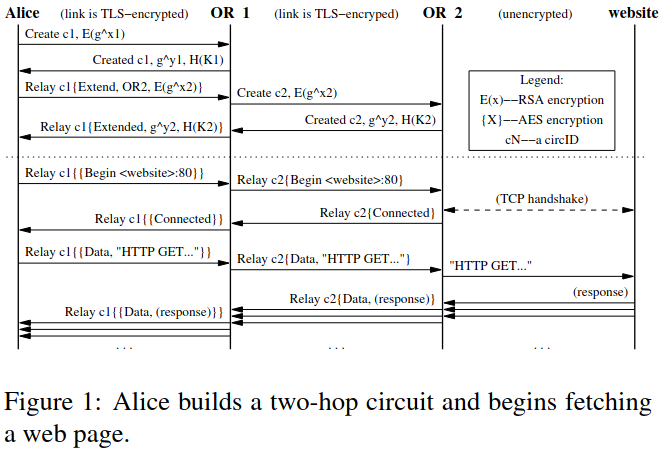
\includegraphics[heigth=0.9\textheight]{../encap/tor-fig1}}
\end{frame}

\begin{frame}{traffic analysis problem}
    \begin{itemize}
    \item problem 1: if I see A send 1000 bytes, then receive 1749 bytes, and\ldots
    \item at about the same time I see B receive 1000 bytes, then send 1749 bytes
    \item \ldots would be a big tell
    \vspace{.5cm}
    \item worse: B or OR 1 or OR 3 can deliberately generate patterns of traffic to help ID A
    \end{itemize}
\end{frame}

\begin{frame}{mitigations for traffic analysis?}
    \begin{itemize}
    \item general idea: add data or delay to make everything `the same'
    \item add padding to traffic sent on `circuit'
        \begin{itemize}
        \item 512-byte cells only (can't see exact sizes in bytes)
        \item additional padding cells added, too
        \end{itemize}
    \item ``cover traffic'' sent periodically between A and OR1
        \begin{itemize}
        \item 1.5 s to 9.5 s in each direction if no traffic
        \item idea: hard for attacker to tell when user active
        \end{itemize}
    \item but real-time nature limits possible mitigations
        \begin{itemize}
        \item similar idea for email avoids with random delays
        \item \ldots but can't really browse the web that way
        \end{itemize}
    \end{itemize}
\end{frame}

\begin{frame}{application-layer tells}
    \begin{itemize}
    \item browser reveals a lot of information:
        \begin{itemize}
        \item browser, OS version
        \item screen size
        \item fonts available
        \item timezone
        \item \ldots
        \end{itemize}
    \item problematic for anonymity
        \begin{itemize}
        \item helps B limit possible other ends very seriously
        \end{itemize}
    \vspace{.5cm}
    \item Tor browser (modified Firefox, essentially) mitigation: \\
        limited set of screen sizes, OS versions, fonts, etc. allowed
    \end{itemize}
\end{frame}

\begin{frame}{other Tor browser paranoia}
    \begin{itemize}
    \item scripts disabled by default
        \begin{itemize}
        \item seriously limits `ordinary' browser security vulnerabilities
        \end{itemize}
    \item cookies, caches cleared when browser closed
    \item HTTPS-only by default
        \begin{itemize}
        \item really dangerous otherwise since we don't trust last onion router
        \end{itemize}
    \end{itemize}
\end{frame}
 % FIXME: incomplete

\section{network layer granularity}

\againframe<4>{encapOpt}

% FIXME:
    % problem: need to run window-size protocol twice
    % only support clever transport stuff (example: SACK)
        % if all parties do
    % (but could do clever transport stuff local to proxy)
    % if we tunnel IP packets, no need to redo that

% FIXME: slide for connect one machie use-case

\subsection{GRE}

\againframe<2>{connTwoNet}

\usetikzlibrary{arrows.meta,calc,patterns,shapes}
\providecommand{\computer}{%
    
\includegraphics[width=1cm]{../common/Noun_project_216.pdf}
}
\providecommand{\switch}{%
    
\includegraphics[width=0.9cm]{../common/fig-switch.pdf}
}
\providecommand{\bigswitch}{%
    
\includegraphics[width=1.4cm]{../common/fig-switch.pdf}
}
\providecommand{\router}{%
    
\includegraphics[width=0.9cm]{../common/fig-router.pdf}
}


\begin{frame}[fragile,label=greSeg]{GRE segment format}
\begin{tikzpicture}
    \tikzset{
        box/.style={draw,thick},
        box unused/.style={draw,thick,pattern=north west lines},
        box label/.style={midway,font=\small,align=center},
        box label flags/.style={midway,font=\fontsize{8}{9}\selectfont,align=center},
        hi on/.style={alt=<#1>{ultra thick,fill=red!10}},
        explain box 1/.style={draw=red,line width=0.8mm,fill=white,anchor=center,at={(explain box loc 1)},align=center},
        explain box 2/.style={draw=red,line width=0.8mm,fill=white,anchor=center,at={(explain box loc 2)},align=center},
        explain box 3/.style={draw=red,line width=0.8mm,fill=white,anchor=center,at={(explain box loc 3)},align=center},
    }
    \begin{scope}[x=4.7mm,y=9mm]
        \coordinate (explain box loc 1) at (16, -3.1);
        \coordinate (explain box loc 2) at (16, -5.1);
        \coordinate (explain box loc 3) at (16, -1.1);
        \path[shading=axis,top color=white,bottom color=black!20] (0, 1) rectangle (32, 0)
            node[box label] {(IP or UDP header (for tunnel))};
        \path[box,hi on=2] (0, 0) rectangle ++(1, -1) node[box label flags] {C};
        \path[box,hi on=0] (1, 0) rectangle ++(1, -1) node[box label flags] {0};
        \path[box,hi on=2,hi on=3] (2, 0) rectangle ++(1, -1) node[box label flags] {K};
        \path[box,hi on=2] (3, 0) rectangle ++(1, -1) node[box label flags] {S};
        \path[box,hi on=0] (4, 0) rectangle (12, -1) node[box label] {0};
        \path[box,hi on=0] (12, 0) rectangle (16, -1) node[box label] {vers\\0};
        \path[box,hi on=0] (16, 0) rectangle (32, -1) node[box label] {protocol type \\ (EtherType)};
        \path[box,hi on=0] (0, -1) rectangle (16, -2) node[box label] {checksum (if C set)};
        \path[box,hi on=0] (16, -1) rectangle (32, -2) node[box label] {0 (if C set)};
        \path[box,hi on=0,hi on=3] (0, -2) rectangle (32, -3) node[box label] {key (if K set)};
        \path[box,hi on=0] (0, -3) rectangle (32, -4) node[box label] {sequence number (if S set)};
        \path[overlay,shading=axis,top color=black!20,bottom color=white] (0, -4) rectangle (32, -5)
            node[box label] {
                encapsulated header+data \\
                (probably IPv4 or IPv6)
            };
        \begin{visibleenv}<2>
            \node[explain box 2] {
                checksum, `key' ($\sim$ port), sequence number optional
            };
        \end{visibleenv}
        \begin{visibleenv}<3>
            \node[explain box 2] {
                key to allow multiple connections \\
                if over UDP, could use separate ports instead \\
                (but usualy not over UDP)
            };
        \end{visibleenv}
    \end{scope}
\end{tikzpicture}
\end{frame}


\subsection{adding encryption/authentication}
\begin{frame}{encapsulatoin with encryption}
    \begin{itemize}
    \item GRE = sends packets as is, setup in advance
    \vspace{.5cm}
    \item often want to add autoconfiguration + encryption + authentication
    \item typically:
        \begin{itemize}
        \item TLS-handshake like \textit{key exchange} protocol to setup conncetion
        \item add space for message authentication code, nonce
        \item encrypt data with symmetric keys
        \end{itemize}
    \item example protocols:
        \begin{itemize}
        \item IKE (setup/key exchange) + IPsec ESP (actual tunnel)
        \item OpenVPN (both)
        \item WireGuard (both)
        \end{itemize}
    \end{itemize}
\end{frame}


\subsection{issues with over TCP}
\begin{frame}{TCP-in-TCP problems}
    \begin{itemize}
    \item sometimes run IP tunnel over TCP
        \begin{itemize}
        \item example: picky firewall rules, or non-UDP-supporting NAT
        \end{itemize}
    \item outer TCP connection adds extra buffering
        \begin{itemize}
        \item more than UDP, because will usually buffer instead of dropping
        \end{itemize}
    \vspace{.5cm}
    \item $\rightarrow$ very high round-trip time if not careful
    \item can result in very poor TCP performance
    \end{itemize}
\end{frame}


\section{link-layer granularity}

\againframe<2>{connTwoNet}

\subsection{VLANs}

\begin{frame}{VLAN idea}
    \begin{itemize}
    \item multiple (`virtual') local networks over one network
    \item links/ports either shared or assigned to just one network
    \item most common implementation: Ethernt 802.1q:
    \vspace{.5cm}
    \item on shared links, frames tagged with their `VLAN ID'
        \begin{itemize}
        \item special case: untagged frames part of VLAN ID 0x0
        \end{itemize}
    \item tags added/removed when going to unshared links
        \begin{itemize}
        \item and broadcast frames filtered out if VLAN ID doesn't match
        \end{itemize}
    \end{itemize}
\end{frame}

\begin{frame}[fragile]{Ethernet encapsulation}
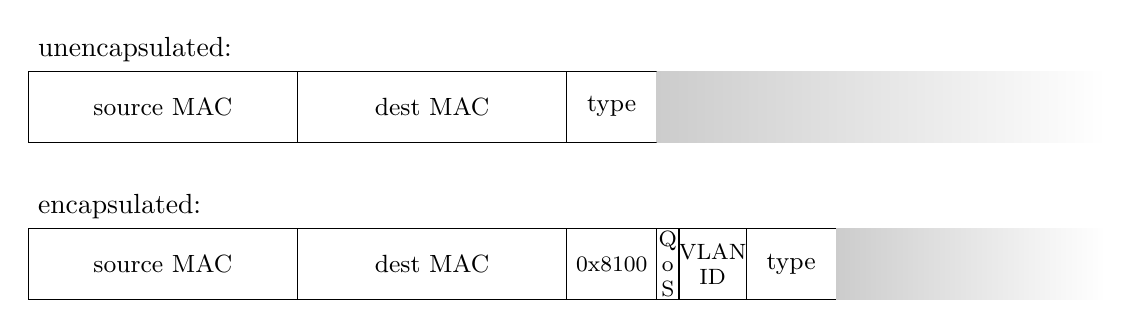
\begin{tikzpicture}
    \tikzset{
        box/.style={draw,thick},
        box unused/.style={draw,thick,pattern=north west lines},
        box label/.style={midway,font=\small,align=center},
        box label flags/.style={midway,font=\fontsize{8}{9}\selectfont,align=center},
        hi on/.style={alt=<#1>{ultra thick,fill=red!10}},
        explain box 1/.style={draw=red,line width=0.8mm,fill=white,anchor=center,at={(explain box loc 1)},align=center},
        explain box 2/.style={draw=red,line width=0.8mm,fill=white,anchor=center,at={(explain box loc 2)},align=center},
        explain box 3/.style={draw=red,line width=0.8mm,fill=white,anchor=center,at={(explain box loc 3)},align=center},
    }
    \begin{scope}[x=5.7mm,y=9mm]
        \node[anchor=south west] at (0, 0) {unencapsulated:};
        \coordinate (explain box loc 1) at (16, -6.1);
        \draw (0, 0) rectangle ++(6, -1) node[box label]{source MAC};
        \draw (6, 0) rectangle ++(6, -1) node[box label]{dest MAC};
        \draw (12, 0) rectangle ++(2, -1) node[box label]{type};
        \path[shading=axis,right color=white, left color=black!20] (14, 0) rectangle (24, -1);
    \end{scope}
    \begin{scope}[x=5.7mm,y=9mm,yshift=-2cm]
        \node[anchor=south west] at (0, 0) {encapsulated:};
        \draw (0, 0) rectangle ++(6, -1) node[box label]{source MAC};
        \draw (6, 0) rectangle ++(6, -1) node[box label]{dest MAC};
        \draw (12, 0) rectangle ++(2, -1) node[box label flags]{0x8100};
        \draw (14, 0) rectangle ++(.5, -1) node[box label flags]{Q\\o\\S};
        \draw (14.5, 0) rectangle ++(1.5, -1) node[box label flags]{VLAN\\ID};
        \draw (16, 0) rectangle ++(2, -1) node[box label]{type};
        \path[shading=axis,right color=white, left color=black!20] (18, 0) rectangle (24, -1);
    \end{scope}
\end{tikzpicture}
\begin{itemize}
    \item encapsulation typically added/removed by switches
        \begin{itemize}
        \item sysadmin configures specific ports to be on a VLAN
        \item another common case: virtual machine software
        \end{itemize}
    \item network IDs (`VLAN identifiers') configured by sysadmins
        \begin{itemize}
        \item special case: 0x0 = default (untagged), 0xFFF = reserved
        \end{itemize}
    \item usually increase in supported frame size to accomodate tag
\end{itemize}
\end{frame}



\subsection{MPLS}

\usetikzlibrary{arrows.meta,calc,matrix,patterns,shapes}
\providecommand{\computer}{%
    
\includegraphics[width=1cm]{../common/Noun_project_216.pdf}
}
\providecommand{\switch}{%
    
\includegraphics[width=0.9cm]{../common/fig-switch.pdf}
}
\providecommand{\bigswitch}{%
    
\includegraphics[width=1.4cm]{../common/fig-switch.pdf}
}
\providecommand{\router}{%
    
\includegraphics[width=0.9cm]{../common/fig-router.pdf}
}



\begin{frame}[fragile]{multiprotocol label switching (MPLS)}
    \begin{itemize}
    \item MPLS: combines encapsulation and routing tables
    \end{itemize}
\begin{tikzpicture}
\tikzset{
    box/.style={draw,thick},
    box unused/.style={draw,thick,pattern=north west lines},
    box label/.style={midway,font=\small,align=center},
    computer/.style={inner sep=0mm,outer sep=0mm,execute at begin node={\computer}},
    switch/.style={inner sep=0mm,outer sep=0mm,execute at begin node={\switch}},
    router/.style={inner sep=-.5mm,outer sep=0mm,execute at begin node={\router}},
    port/.style={pos=0.95,fill=white,circle,draw,inner sep=0mm},
    port beginning/.style={pos=0.05,fill=white,circle,draw,inner sep=0mm},
    box label flags/.style={midway,font=\fontsize{8}{9}\selectfont,align=center},
    hi on/.style={alt=<#1>{ultra thick,fill=red!10}},
    explain box 1/.style={draw=red,line width=0.8mm,fill=white,anchor=center,at={(explain box loc 1)},align=center},
    explain box 2/.style={draw=red,line width=0.8mm,fill=white,anchor=center,at={(explain box loc 2)},align=center},
    explain box 3/.style={draw=red,line width=0.8mm,fill=white,anchor=center,at={(explain box loc 3)},align=center},
    route table/.style={
        matrix of nodes,ampersand replacement=\&,
        column sep=-.3mm, row sep=-.3mm,
        nodes={align=center,font=\fontsize{9}{10}\selectfont\tt,text depth=1mm,text height=3mm,minimum height=0.4cm,inner sep=0mm,draw,line width=.3mm},
        column 1/.style={nodes={text width=.7cm}},
        column 2/.style={nodes={text width=0.7cm}},
        column 3/.style={nodes={text width=1.7cm,font=\fontsize{7}{8}\selectfont\tt}},
        column 4/.style={nodes={text width=1.5cm}},
        column 5/.style={nodes={text width=.5cm}},
        row 1/.style={nodes={draw=none,font=\fontsize{9}{10}\selectfont}},
    },
    route table no in no dest/.style={
        matrix of nodes,ampersand replacement=\&,
        column sep=-.3mm, row sep=-.3mm,
        nodes={align=center,font=\fontsize{9}{10}\selectfont\tt,text depth=1mm,text height=3mm,minimum height=0.4cm,inner sep=0mm,draw,line width=.3mm},
        column 1/.style={nodes={text width=0.7cm}},
        column 2/.style={nodes={text width=1.5cm}},
        column 3/.style={nodes={text width=.5cm}},
        row 1/.style={nodes={draw=none,font=\fontsize{9}{10}\selectfont}},
    },
    route table no dest no in/.style={route table no in no dest},
    connect/.style={draw,very thick},
    msg/.style={
        matrix of nodes,nodes={draw,violet,line width=.3mm,font=\fontsize{8}{9}\selectfont\tt,
            inner sep=0mm,inner xsep=.5mm,text height=3mm,text depth=.5mm},
        fill=white,
        column sep=-.3mm,inner sep=0mm
    },
    >=Latex,
    hi row/.style 2 args={
        alt=<#1>{
            row #2/.style={nodes={fill=red!15}}
        }
    },
}
\node[router] (in0) at (0, 6) {};
\draw[connect,->] (-1, 7) -- (in0.north west) node[port]{0};
%\draw[connect,->] (-1, 6) -- (in0.west) node[port]{1};
\matrix[route table,anchor=north,hi row={2}{2}] at (0, 5.5) {
in \& label \& dest \& op \& out \\
0\& --- \& 3fff:1::/32 \& push 4 \& 2 \\
0 \& --- \& 3fff:2::/32 \& push 7 \& 2 \\
2 \& 9 \& --- \& pop \& 0\\
\ldots \& \ldots \& \ldots \& \ldots \& \ldots \\
};
\node[router] (out0) at (10, 8) {};
\draw[connect,->] (out0.east) -- ++(.5, 0) node[right,font=\tiny\tt] {3fff:1::/32}
    node[port beginning] {1};
\draw[connect,->] (out0.north east) -- ++(.5, .5)
    node[port beginning] {2};
\node[router] (out1) at (5, 4) {};
\draw[connect,->] (out1.south) -- ++(0, -.5) node[right,font=\tiny\tt] {3fff:2::/32}
    node[port beginning] {1};
\node[router,alt=<5>{fill=red!10}] (mid1) at (5, 6) {};
\matrix[alt=<5>{draw=red,very thick},route table no in no dest,anchor=south,hi row={2-4}{2}] (mid1 table) at ([xshift=-1.5cm]mid1.north) {
label \& op \& out \\
24 \& swap 1 \& 21 \\
25 \& swap 2 \& 21 \\
27 \& swap 1 \& 22 \\
28 \& swap 9 \& 0 \\
\ldots \& \ldots \& \ldots \\
};
\matrix[route table,anchor=north,hi row={2}{4}] at ([yshift=-.3cm]out0.south) {
in \& label \& dest \& op \& out \\
1 \& --- \& 3fff:2::/32\& push 27 \& 0\\
1 \& --- \& default \& push 28 \& 0\\
0 \& 21 \& --- \& pop \& 21 \\
0 \& 22 \& --- \& pop \& 22 \\
\ldots \& \ldots \& \ldots \& \ldots \& \ldots \\
};
\foreach \x/\y/\xp/\yp in {in0/mid1/2/0,mid1/out0/1/0,mid1/out1/2/0} {
    \draw[connect,<->] (\x) -- (\y) node[port beginning] {\xp} node[port] {\yp};
}
\begin{visibleenv}<2-4>
    \matrix[msg,anchor=south] at ([yshift=.5cm]in0.north west) {
        dest=3fff:1::aa \& \ldots \\
    };
    \matrix[msg,anchor=west] at ([xshift=.5cm]in0.east) {
        |[alt={<3>{fill=red!15}}]| 24 \& dest=3fff:1::aa \& \ldots \\
    };
    \matrix[msg,anchor=west] at ([xshift=.5cm,yshift=1cm]mid1.east) {
        |[alt={<3>{fill=red!15}}]| 21 \& dest=3fff:1::aa \& \ldots \\
    };
\end{visibleenv}
\begin{visibleenv}<3>
\node[align=left,draw=red,very thick,fill=white,anchor=west] at (mid1 table.east) {
    `swap' operation to translate \\
    between different label meanings \\
    ~ \\
    allows piecemail configuration
};
\end{visibleenv}
\begin{visibleenv}<5>
\node[align=left,draw=red,very thick,fill=white,anchor=west] at (mid1 table.east) {
    routers in `middle' of network \\
    have \textit{very simple} routing decisions \\
    no prefix matching
};
\end{visibleenv}
\end{tikzpicture}
\end{frame}

\begin{frame}{Label Distribution Protocol}
    \begin{itemize}
    \item share with neighbors list of:
        \begin{itemize}
        \item (ultimate destination, desired label)
        \end{itemize}
    \item use entries to
        \begin{itemize}
        \item allocate new local labels
        \item setup appropriate \texttt{swap} entries
        \item send other neighbors update about new labels
        \end{itemize}
    \vspace{.5cm}
    \item if using normal routing protocol to decide which neighbors routes to accept,
    just a funny way to implement routing tables
    \end{itemize}
\end{frame}

\begin{frame}[fragile]{MPLS tunnel}
\begin{tikzpicture}
\tikzset{
    box/.style={draw,thick},
    box unused/.style={draw,thick,pattern=north west lines},
    box label/.style={midway,font=\small,align=center},
    computer/.style={inner sep=0mm,outer sep=0mm,execute at begin node={\computer}},
    switch/.style={inner sep=0mm,outer sep=0mm,execute at begin node={\switch}},
    router/.style={inner sep=-.5mm,outer sep=0mm,execute at begin node={\router}},
    port/.style={pos=0.95,fill=white,circle,draw,inner sep=0mm},
    port beginning/.style={pos=0.05,fill=white,circle,draw,inner sep=0mm},
    box label flags/.style={midway,font=\fontsize{8}{9}\selectfont,align=center},
    hi on/.style={alt=<#1>{ultra thick,fill=red!10}},
    explain box 1/.style={draw=red,line width=0.8mm,fill=white,anchor=center,at={(explain box loc 1)},align=center},
    explain box 2/.style={draw=red,line width=0.8mm,fill=white,anchor=center,at={(explain box loc 2)},align=center},
    explain box 3/.style={draw=red,line width=0.8mm,fill=white,anchor=center,at={(explain box loc 3)},align=center},
    route table/.style={
        matrix of nodes,ampersand replacement=\&,
        column sep=-.3mm, row sep=-.3mm,
        nodes={align=center,font=\fontsize{9}{10}\selectfont\tt,text depth=1mm,text height=3mm,minimum height=0.4cm,inner sep=0mm,draw,line width=.3mm},
        column 1/.style={nodes={text width=.7cm}},
        column 2/.style={nodes={text width=0.7cm}},
        column 3/.style={nodes={text width=1.7cm,font=\fontsize{7}{8}\selectfont\tt}},
        column 4/.style={nodes={text width=1.5cm}},
        column 5/.style={nodes={text width=.5cm}},
        row 1/.style={nodes={draw=none,font=\fontsize{9}{10}\selectfont}},
    },
    route table no in no dest/.style={
        matrix of nodes,ampersand replacement=\&,
        column sep=-.3mm, row sep=-.3mm,
        nodes={align=center,font=\fontsize{9}{10}\selectfont\tt,text depth=1mm,text height=3mm,minimum height=0.4cm,inner sep=0mm,draw,line width=.3mm},
        column 1/.style={nodes={text width=0.7cm}},
        column 2/.style={nodes={text width=1.5cm}},
        column 3/.style={nodes={text width=.5cm}},
        row 1/.style={nodes={draw=none,font=\fontsize{9}{10}\selectfont}},
    },
    route table no dest/.style={
        matrix of nodes,ampersand replacement=\&,
        column sep=-.3mm, row sep=-.3mm,
        nodes={align=center,font=\fontsize{9}{10}\selectfont\tt,text depth=1mm,text height=3mm,minimum height=0.4cm,inner sep=0mm,draw,line width=.3mm},
        column 1/.style={nodes={text width=0.7cm}},
        column 2/.style={nodes={text width=0.7cm}},
        column 3/.style={nodes={text width=1.5cm}},
        column 4/.style={nodes={text width=.5cm}},
        row 1/.style={nodes={draw=none,font=\fontsize{9}{10}\selectfont}},
    },
    route table no dest no in/.style={route table no in no dest},
    connect/.style={draw,very thick},
    msg/.style={
        matrix of nodes,nodes={draw,violet,line width=.3mm,font=\fontsize{8}{9}\selectfont\tt,
            inner sep=0mm,inner xsep=.5mm,text height=3mm,text depth=.5mm},
        fill=white,
        column sep=-.3mm,inner sep=0mm},
    >=Latex,
    hi row/.style 2 args={
        alt=<#1>{
            row #2/.style={nodes={fill=red!15}}
        }
    },
}

\node at (6, 9) {logical view --- `virtual wire'};
\node (log A) at (-2, 8.5) {A};
\node (log B) at (13, 8.5) {B};
\draw[connect,<->] (log A) -- (log B);

\draw[overlay, ultra thick] (-3.5, 7.8) -- (14, 7.8);

\node[anchor=north] at (6, 7.8) {actual network};

\node[router] (in0) at (0, 6) {};
\draw[connect,<->] (-1.5, 6) -- (in0.west) node[port]{0}
    node[pos=0,left] {A};
\matrix[route table no dest,anchor=north] at (0, 5.5) {
in \& label  \& op \& out \\
0 \& ---  \& push 32 \& 1 \\
--- \& 1 \& pop \& 0 \\
\ldots \& \ldots \& \ldots \& \ldots \\
};
\node[router] (mid1) at (4, 6) {};
\matrix[route table no dest no in,anchor=north] at (4, 4) {
label  \& op \& out \\
32 \& swap 37 \& 4 \\
26 \& swap 21 \& 0 \\
\ldots \& \ldots \& \ldots \\
};
\node[router] (mid2) at (8, 6) {};
\matrix[route table no dest no in,anchor=north] at (8, 5.5) {
label  \& op \& out \\
37 \& swap 20 \& 6 \\
39 \& swap 32 \& 3 \\
\ldots \& \ldots \& \ldots \\
};
\node[router] (out0) at (11, 6) {};
\matrix[route table no dest,anchor=north] at (11, 4) {
in \& label  \& op \& out \\
0 \& --- \& push 37 \& 1 \\
--- \& 0 \& swap 29 \& 6 \\
\ldots \& \ldots \& \ldots \& \ldots \\
};
\draw[connect,->](out0.east) -- ++(1, 0) node[port beginning]{0}
    node[pos=1,right] {B};

\foreach \x/\y in {mid1/30,mid1/60,mid1/270,mid2/45,mid2/90,mid2/210,mid2/290,
                   in0/90,in0/270,out0/60,out0/280} {
    \draw[connect,<-] (\x.\y) -- ++(\y:.5cm);
};
\foreach \x/\y/\xp/\yp in {in0/mid1/1/0,mid1/mid2/4/3,mid2/out0/6/1} {
    \draw[connect,<->] (\x) -- (\y) node[port beginning] {\xp} node[port] {\yp};
}
\end{tikzpicture}
\end{frame}

\begin{frame}{MPLS tunnels for traffic engineering}
    \begin{itemize}
    \item if multiple paths from A to B often want to:
        \begin{itemize}
        \item balance between them to use available bandwidth
        \item prioritize important traffic on `better' path
        \item \ldots
        \end{itemize}
    \item plain OSPF can't really do any of this unless equal cost
    \vspace{.5cm}
    \item MPLS gives mechanism to do this kind of balancing:
        \begin{itemize}
        \item setup labels along desired paths
        \item choosing new path (or failover) = changing `swap X' to `swap Y'
        \item can configure backup paths in advance and turn them on later
        \end{itemize}
    \end{itemize}
\end{frame}

\begin{frame}[fragile]{rapid failover}
\begin{tikzpicture}
\tikzset{
    box/.style={draw,thick},
    box unused/.style={draw,thick,pattern=north west lines},
    box label/.style={midway,font=\small,align=center},
    computer/.style={inner sep=0mm,outer sep=0mm,execute at begin node={\computer}},
    switch/.style={inner sep=0mm,outer sep=0mm,execute at begin node={\switch}},
    router/.style={inner sep=-.5mm,outer sep=0mm,execute at begin node={\router}},
    port/.style={pos=0.95,fill=white,circle,draw,inner sep=0mm},
    port beginning/.style={pos=0.05,fill=white,circle,draw,inner sep=0mm},
    box label flags/.style={midway,font=\fontsize{8}{9}\selectfont,align=center},
    hi on/.style={alt=<#1>{ultra thick,fill=red!10}},
    explain box 1/.style={draw=red,line width=0.8mm,fill=white,anchor=center,at={(explain box loc 1)},align=center},
    explain box 2/.style={draw=red,line width=0.8mm,fill=white,anchor=center,at={(explain box loc 2)},align=center},
    explain box 3/.style={draw=red,line width=0.8mm,fill=white,anchor=center,at={(explain box loc 3)},align=center},
    route table/.style={
        matrix of nodes,ampersand replacement=\&,
        column sep=-.3mm, row sep=-.3mm,
        nodes={align=center,font=\fontsize{9}{10}\selectfont\tt,text depth=1mm,text height=3mm,minimum height=0.4cm,inner sep=0mm,draw,line width=.3mm},
        column 1/.style={nodes={text width=.7cm}},
        column 2/.style={nodes={text width=0.7cm}},
        column 3/.style={nodes={text width=1.7cm,font=\fontsize{7}{8}\selectfont\tt}},
        column 4/.style={nodes={text width=1.5cm}},
        column 5/.style={nodes={text width=.5cm}},
        row 1/.style={nodes={draw=none,font=\fontsize{9}{10}\selectfont}},
    },
    route table no in no dest/.style={
        matrix of nodes,ampersand replacement=\&,
        column sep=-.3mm, row sep=-.3mm,
        nodes={align=center,font=\fontsize{9}{10}\selectfont\tt,text depth=1mm,text height=3mm,minimum height=0.4cm,inner sep=0mm,draw,line width=.3mm},
        column 1/.style={nodes={text width=0.7cm}},
        column 2/.style={nodes={text width=1.5cm}},
        column 3/.style={nodes={text width=.5cm}},
        row 1/.style={nodes={draw=none,font=\fontsize{9}{10}\selectfont}},
    },
    route table no dest/.style={
        matrix of nodes,ampersand replacement=\&,
        column sep=-.3mm, row sep=-.3mm,
        nodes={align=center,font=\fontsize{9}{10}\selectfont\tt,text depth=1mm,text height=3mm,minimum height=0.4cm,inner sep=0mm,draw,line width=.3mm},
        column 1/.style={nodes={text width=0.7cm}},
        column 2/.style={nodes={text width=0.7cm}},
        column 3/.style={nodes={text width=1.5cm}},
        column 4/.style={nodes={text width=.5cm}},
        row 1/.style={nodes={draw=none,font=\fontsize{9}{10}\selectfont}},
    },
    route table no dest no in/.style={route table no in no dest},
    connect/.style={draw,very thick},
    msg/.style={
        matrix of nodes,nodes={draw,violet,line width=.3mm,font=\fontsize{8}{9}\selectfont\tt,
            inner sep=0mm,inner xsep=.5mm,text height=3mm,text depth=.5mm},
        fill=white,
        column sep=-.3mm,inner sep=0mm},
    >=Latex,
    hi row/.style 2 args={
        alt=<#1>{
            row #2/.style={nodes={fill=red!15}}
        }
    },
}

\draw[connect,<->] (-1.5, 6) -- (in0.west) node[port]{0}
\node[router] (in0) at (0, 6) {};
\matrix[route table no dest no  in,anchor=north] at (0, 5.5) {
label  \& op \& out \\
21 \& swap 25 \& 1 \\
(backup) 21 \& swap 27 \& 2 \\
27 \& swap 30 \& 0 \\
 \ldots \& \ldots \& \ldots \\
};
\node[router] (mid1) at (12, 6) {};
\matrix[route table no dest no in,anchor=north] at (12, 5.5) {
label  \& op \& out \\
25 \& swap 27 \& 3 \\ 
 \ldots \& \ldots \& \ldots \\
};
\node[router] (out0) at (6, 4) {};
\matrix[route table no dest no in,anchor=north] at (6, 3.5) {
label  \& op \& out \\
27 \& swap 24 \& 3 \\
28 \& swap 25 \& 1 \\
\ldots \& \ldots \& \ldots \\
};
\draw[connect,<->] (-13.5, 6) -- (out0.east) node[port]{1}
\foreach \x/\y/\xp/\yp in {in0/out0/1/1,in0/mid1/2/1,mid1/out0/3/2} {
    \draw[connect,<->] (\x) -- (\y) node[port beginning] {\xp} node[port] {\yp};
}
\end{tikzpicture}
\end{frame}

\begin{frame}{RSVP-TE}
    \begin{itemize}
    \item RSVP-TE (RFC 3209): protocol for setting up MPLS tunnels
    \item idea: routers figure out labels, etc.
    \item end-user can (optionally) specify\ldots
    \vspace{.5cm}
    \item that tunnel go through specific routers
    \item also setting up `fast reroute' backup paths
    \item bandwidth reservation 
        \begin{itemize}
        \item routers give you error if bandwidth not gaurenteed
        \end{itemize}
    \end{itemize}
\end{frame}

\begin{frame}{nested labels}
    \begin{itemize}
    \item label \textit{stack} allows \ldots
    \item nested tunnels
    \item marking different types of packet
    \item \ldots
    \end{itemize}
\end{frame}

\begin{frame}{protocol-independence}
    \begin{itemize}
    \item only first/last routers care about actual protocol
    \item easily allows for\ldots
    \vspace{.5cm}
    \item mix of Ethernet and IP tunnels
    \item using routers that don't support IP (e.g. ATM)
    \item \ldots
    \end{itemize}
\end{frame}

\begin{frame}[fragile]{actual label format}
\begin{Verbatim}[fontsize=\small]
 0                   1                   2                   3
 0 1 2 3 4 5 6 7 8 9 0 1 2 3 4 5 6 7 8 9 0 1 2 3 4 5 6 7 8 9 0 1
+-+-+-+-+-+-+-+-+-+-+-+-+-+-+-+-+-+-+-+-+-+-+-+-+-+-+-+-+-+-+-+-+ Label
|                Label                  | Exp |S|       TTL     | Stack
+-+-+-+-+-+-+-+-+-+-+-+-+-+-+-+-+-+-+-+-+-+-+-+-+-+-+-+-+-+-+-+-+ Entry

                    Label:  Label Value, 20 bits
                    Exp:    Experimental Use, 3 bits
                    S:      Bottom of Stack, 1 bit
                    TTL:    Time to Live, 8 bits
\end{Verbatim}
\begin{itemize}
\item TTL here is different than we've seen:
\item only processed when label popped
\item typically (re)set to mirror IP TTL if MPLS run over IP
\end{itemize}
\end{frame}




\section{encapsulation costs}
\begin{frame}{encapsulation overheads}
\begin{tabular}{l||p{4cm}|p{4cm}|p{2cm}}
left in above       & TCP/UDP/higher layers & IP & link-layer \\ \hline \hline
above TCP/UDP       & HTTP proxy, DNS over HTTP(S) & --- & --- \\ \hline
TCP/UDP             & SOCKS, HTTP CONNECT, SSH conn forwarding, TLS & --- & --- \\\hline
IP                  & OpenVPN, WireGuard & GRE, IPsec & MPLS \\\hline
link-layer          & OpenVPN, \ldots & ? & VLAN, MPLS \\\hline
\end{tabular}
\begin{itemize}
\item which of these types of options\ldots
    \begin{itemize}
    \item best for throughput?
    \item best for latency?
    \item best if both ends are behind a NAT?
    \item bets for compatibility?
    \end{itemize}
\end{itemize}
\end{frame}


\section{which encapsulation for}
\begin{frame}{which encapuslation (1)}
    \begin{itemize}
    \item suppose I have two racks of servers in two different buildings
    \item want them to be in the same subnetwork
        \begin{itemize}
        \item so they'll find each other with broadcast, multicast DNS
        \end{itemize}
    \item how should I do this if\ldots
        \begin{itemize}
        \item the two buildings are connected via Ethernet also used for internet access?
        \item the two buildings are connected via an IP link leased from an ISP?
        \end{itemize}
    \end{itemize}
\end{frame}

\begin{frame}{which encapuslation (2)}
    \begin{itemize}
    \item suppose I have a rack of servers in my building, but I'm migrating to the cloud
    \item I've moved one server to a cloud provider\ldots
    \item I don't want to reconfigure the other servers that talk to it\ldots
    \vspace{.5cm}
    \item what would be some options to do this? what else do we need to know about the server?
    \item what would be useful features for cloud provider to give us?
    \end{itemize}
\end{frame}

\begin{frame}{which encapsulation (3)}
    \begin{itemize}
    \item I need to have my machines which handle payment processing go be behind a firewall
    \item but they're in the same rack as machines which should have a direct internet connection
    \vspace{.5cm}
    \item how should I do this?
    \end{itemize}
\end{frame}

